	\newpage
\section{Potential Telescopes for Spectroscopy Strategy} % (fold)
	\label{sub:candidate_telescopes}
		\subsection{James Webb Space Telescope} % (fold)
		\label{ssub:james_webb_space_telescope}
			The primary telescopes considered for use in this research are the JWST and the E-ELT. The JWST's NIRSpec is a device which will enable the conformation of high red shift galaxies. It uses a combination of slits, prims and gratings to achieve high resolution spectroscopy. Perhaps its most innovative feature is a microshutter array. The microshutters are tiny cells that measure $100 \times 200$\,\si{\micro\metre}. They are arranged over a waffle like grid containing \num{62000} individual cells. NIRSpec will contain four identical grids in total. The cells all have lids which can be opened and closed individually. This is achieved by sweeping a magnet across the surface of the array which opens all of the lids and the electronically closing individual lids. Each cell measures $203 \times 463$\,milliarcseconds. The total field of view for all four arrays combined is $3 \times 3$\,arcminutes. Shutters in each array can be opened or closed to form multiple apertures meaning that spectrums for one hundred different targets can be found simultaneously. The size and shape of the apertures can be selected to obtain the clearest spectrum possible for each individual target. Figures~\ref{fig:nirspec_construction} and~\ref{fig:nirspec_mirrors} show NIRSpec under construction\cite{NIRSpec}\cite{JWSTinformation}.
			\begin{figure}[htbp]
				\begin{minipage}[c]{0.5\linewidth}
					\centering
					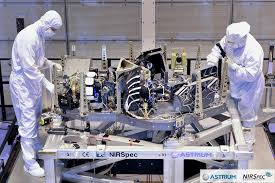
\includegraphics[width=0.9\textwidth]{../Images/nirspec_construction.jpeg}
					\caption{\label{fig:nirspec_construction}}
				\end{minipage}
				\begin{minipage}[c]{0.5\linewidth}
					\centering
					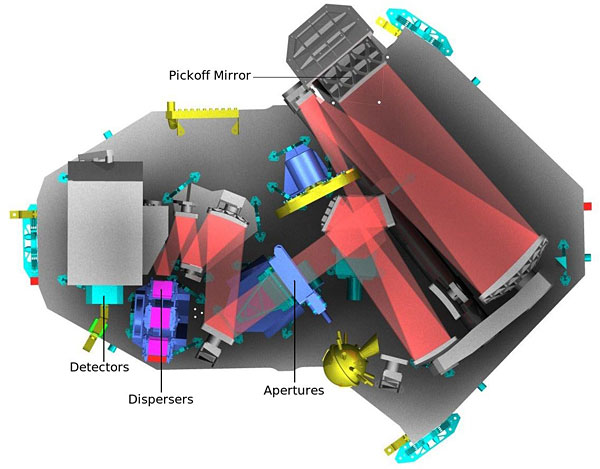
\includegraphics[width=0.9\textwidth]{../Images/nirspec_mirrors.jpeg}
					\caption{\label{fig:nirspec_mirrors}}
				\end{minipage}
			\end{figure}

			As well as the microshutter array the JWST also contains an integral field unit. Integral field spectroscopy has become an important sub discipline of astronomy where there is a need to study the spectra of extended bodies. This has particular significance as high red shift galaxies are considered to be extended bodies.

			Integral field spectroscopy is the successor to long slit spectroscopy where the spectrum is dispersed perpendicular to the slit direction. By stepping the position of the slit the spectrum of points over the extended body can be obtained. An integral field unit speeds up this process by slicing the image and then rearranging it so that different parts can illuminate the slit. This negates the need to take multiple exposures\cite{IntegralJWST}\cite{IntegralSpec}.

			NIRSpec will be able to disperse light comprised of wavelengths between 0.6 and 5 microns, i.e. the infrared range over which the Gunn-Peterson trough should occur. It will do this using one prism and five diffraction gratings. The wavelength ranges over which each will work and their associated wavelengths are shown below\cite{JWSTnumbers}.
			\begin{table}[htbp]
				\begin{center}
					\begin{tabular}{c|c|c|c}
						Grating & Filter & Resolution & Wavelength (\si{\micro\metre}) \\
						\hline \hline
						Prism & Clear & 100 & 0.5--5 \\
						G140M & F100LP & 1000 & 1.0--1.8 \\
						G235M & F170LP & 1000 & 1.7--3.0 \\
						G395M & F290LP & 1000 & 2.9--5.0 \\
						G140M & F100LP & 2700 & 1.0--1.8 \\
						G235M & F170LP & 2700 & 1.7--3.0 \\
						G395M & F290LP & 2700 & 2.9--5.0
					\end{tabular}
				\end{center}
				\caption{Number of galaxies for set total observing time given different magnitudes/ survey areas for JWST.\label{tab:galaxies_for_set_total_observing_time_JWST}}
			\end{table}
		% subsubsection james_webb_space_telescope (end)

		\subsection{European Extremely Large Telescope} % (fold)
		\label{sub:european_extremely_large_telescope}
			The European-Extremely Large Telescope (E-ELT) will be equipped with three spectroscopic devices:
			\begin{enumerate}
				\item EAGLE - A multichannel integral field near infrared spectrograph with multi object adaptive optics;
				\item HARMONI - A wide band field spectrograph;
				\item SIMPLE - Echelle high resolution spectrograph.
			\end{enumerate}
			EAGLE will enable spectrums of multiple galaxies to be obtained simultaneously and thus would be of great benefit for this project. However, as it is only in early development stage information required to perform estimates for exposure times is not available. It is most likely to use a system of fibre optics to stack spectrums of galaxies onto the CCD. The fibre optics will sit between the diffraction grating and the CCD. As mentioned above it will use a system of multi object adaptive objects. This will use separate pieces of a deformable mirror to compensate for distortions across all the objects in its field of view. The correction applied to these mirrors will be determined by atmospheric tomography using guide stars\cite{MultiObjectAOptics}.

			SIMPLE uses an echelle grating in order to achieve resolving powers up to \num{130000}. It will work over a wavelength range of 0.8--2.5\si{\micro\metre}. In order to understand how echelle gratings can achieve such high resolution we must first consider blazing. The fact that diffraction gratings produce multiple spectra of the same object means that they are very inefficient. Most of the light incident upon a grating will fall in the zeroth order which is undispersed. Only about 10\% of the light will be contained within the first order; the higher the order, the less the percentage. To change these proportions the prism must be blazed. This involves tilting the surface of the grooves by some angle known as the blazing angle. This angle is such that a light ray will emerge from the grating as if by reflection. It is therefore possible to direct as much as 70\% of the light in the order of interest. Without exception the spectrum of different orders will overlap causing contamination. The higher the order, the worse the contamination as the angle through which the spectrum is dispersed is greater. However, for this very reason resolution is much improved. Echelle gratings are therefore blazed in such a way that most of the light falls anywhere from the 10th to the 100th order depending on the blazing angle. In order to remove the contamination present at such orders echelle gratings are used in tandem with cross dispersers. These are low dispersion gratings or prisms with a dispersion axis perpendicular to that of the echelle grating. Their function is to separate out the overlap, thus providing an extremely high resolution spectrum\cite{SIMPLEechelle}\cite{Echelleprinc}.

			HARMONI is a visible and near infrared integral field spectrograph with a field of view of $5 \times 10$\,arc\,minutes. It will cover a wavelength range of 0.47\,to \SI{2.45}{\micro\metre} and enable resolving powers from \num{4000} to \num{20000} providing the E-ELT's core spectroscopic capability. HARMONI provides a range of spatial pixel scales which enable the user to configure the instrument of a multitude of science goals. It can adapt to any flavour of adaptive optics and therefore negate any distortions in light from distant galaxies caused by Earth's atmosphere~\ref{ssub:adaptive_optics}. The wavelength ranges of the diffraction gratings can be seen in the table below\cite{HARMONI}\cite{Hstats}.
			\begin{table}[htbp]
				\begin{center}
					\begin{tabular}{c|c|c}
						Band/Grating & Resolution & Wavelength (\si{\micro\metre}) \\
						\hline \hline
						H+K 	& 3900 	& 1.4-2.4 \\
						I+Z+J 	& 3857 	& 0.8-1.4 \\
						K 		& 8800 	& 2.0-2.5 \\
						H 		& 8892 	& 1.5-1.8 \\
						J 		& 8714 	& 1.1-1.4 \\
						I+Z 	& 8809 	& 0.8-1.0 \\
						K 		& High 	& 19174 2.1-2.3 \\
						H 		& High 	& 19176 1.5-1.7 \\
						J 		& High 	& 20500 1.2-1.3 \\
						z 		& 19222 & 0.8-0.9
					\end{tabular}
				\end{center}
				\caption{Number of galaxies for set total observing time given different magnitudes/ survey areas for JWST.\label{tab:galaxies_for_set_total_observing_time_JWST}}
			\end{table}
		% subsection european_extremely_large_telescope (end)
	% subsection candidate_telescopes (end)
